\documentclass[
    xcolor={svgnames,dvipsnames},
    hyperref={colorlinks, citecolor=DeepPink4, linkcolor=DarkRed, urlcolor=DarkBlue}
    ]{beamer}  % for hardcopy add 'trans'

\mode<presentation>
{
  \usetheme{Singapore}
  % or ...
  \setbeamercovered{transparent}
  % or whatever (possibly just delete it)
}



\addtobeamertemplate{navigation symbols}{}{%
    \usebeamerfont{footline}%
    \usebeamercolor[fg]{footline}%
    \hspace{1em}%
    \insertframenumber/\inserttotalframenumber
}



\usepackage{fontspec} 
%\usepackage[xcharter]{newtxmath}
%\setmainfont{XCharter}
\usepackage{unicode-math}
%\setmathfont{XCharter-Math.otf}
\setmonofont{DejaVu Sans Mono}[Scale=MatchLowercase] % provides unicode characters 

\usepackage{tikz}
\usetikzlibrary{matrix, shapes, arrows.meta, positioning, fit, backgrounds, calc}

% \usetikzlibrary{matrix, arrows.meta, positioning, calc, backgrounds}

% for tikz
\usepackage{pgfplots}
\usepgfplotslibrary{fillbetween}
\pgfplotsset{compat=1.16}

\usepackage{varwidth}
\usepackage{minted}
\usemintedstyle{friendly}
\setminted[python]{
  fontsize=\small,
  baselinestretch=1.2,
  bgcolor=codebg,
  linenos=false,
  breaklines=true,
  frame=none
}
\setminted[matlab]{
  fontsize=\small,
  baselinestretch=1.2,
  bgcolor=codebg,
  linenos=false,
  breaklines=true,
  frame=none
}
\setminted[julia]{
  fontsize=\small,
  baselinestretch=1.2,
  bgcolor=codebg,
  linenos=false,
  breaklines=true,
  frame=none
}
%\setminted{mathescape, frame=lines, framesep=3mm}
%\newminted{python}{}
%\newminted{c}{mathescape,frame=lines,framesep=4mm,bgcolor=bg}
%\newminted{java}{mathescape,frame=lines,framesep=4mm,bgcolor=bg}
%\newminted{julia}{mathescape,frame=lines,framesep=4mm,bgcolor=bg}
%\newminted{ipython}{mathescape,frame=lines,framesep=4mm,bgcolor=bg}

\usepackage{graphicx}
\usepackage{amsmath, amssymb, amsthm}
\usepackage{bbm}
\usepackage{mathrsfs}
\usepackage{xcolor}
\usepackage{fancyvrb}


% Quotes at start of chapters / sections
\usepackage{epigraph}  
\renewcommand{\epigraphwidth}{6in}

%% Fonts

%\usepackage[T1]{fontenc}
\usepackage{mathpazo}
%\usepackage{fontspec}
%\defaultfontfeatures{Ligatures=TeX}
%\setsansfont[Scale=MatchLowercase]{DejaVu Sans}
%\setmonofont[Scale=MatchLowercase]{DejaVu Sans Mono}
%\setmathfont{Asana Math}
%\setmainfont{Optima}
%\setmathrm{Optima}
%\setboldmathrm[BoldFont={Optima ExtraBlack}]{Optima Bold}

% Some colors

\definecolor{containerblue}{RGB}{66, 133, 244}
\definecolor{leafgreen}{RGB}{52, 168, 83}
\definecolor{textgray}{RGB}{51, 51, 51}
\definecolor{backgroundgray}{RGB}{248, 249, 250}
\definecolor{codebg}{RGB}{241, 241, 241}
\definecolor{aquamarine}{RGB}{69,139,116}
\definecolor{midnightblue}{RGB}{25,25,112}
\definecolor{darkslategrey}{RGB}{47,79,79}
\definecolor{darkorange4}{RGB}{139,90,0}
\definecolor{dogerblue}{RGB}{24,116,205}
\definecolor{blue2}{RGB}{0,0,238}
\definecolor{bg}{rgb}{0.95,0.95,0.95}
\definecolor{DarkOrange1}{RGB}{255,127,0}
\definecolor{ForestGreen}{RGB}{34,139,34}
\definecolor{DarkRed}{RGB}{139, 0, 0}
\definecolor{DarkBlue}{RGB}{0, 0, 139}
\definecolor{Blue}{RGB}{0, 0, 255}
\definecolor{Brown}{RGB}{165,42,42}


\setlength{\parskip}{1.5ex plus0.5ex minus0.5ex}

%\renewcommand{\baselinestretch}{1.05}
%\setlength{\parskip}{1.5ex plus0.5ex minus0.5ex}
%\setlength{\parindent}{0pt}

% Typesetting code
\definecolor{bg}{rgb}{0.95,0.95,0.95}
\newcommand{\Fact}{\textcolor{Brown}{\bf Fact. }}
\newcommand{\Facts}{\textcolor{Brown}{\bf Facts }}
\newcommand{\keya}{\textcolor{turquois4}{\bf Key Idea. }}
\newcommand{\Factnodot}{\textcolor{Brown}{\bf Fact }}
\newcommand{\Eg}{\textcolor{ForestGreen}{Example. }}
\newcommand{\Egs}{\textcolor{ForestGreen}{Examples. }}
\newcommand{\Ex}{{\bf Ex. }}



\renewcommand{\theFancyVerbLine}{\sffamily
    \textcolor[rgb]{0.5,0.5,1.0}{\scriptsize {\arabic{FancyVerbLine}}}}

\newcommand{\navy}[1]{\textcolor{DarkBlue}{\bf #1}}
\newcommand{\brown}[1]{\textcolor{Brown}{\sf #1}}
\newcommand{\green}[1]{\textcolor{ForestGreen}{\sf #1}}
\newcommand{\blue}[1]{\textcolor{Blue}{\sf #1}}
\newcommand{\emp}[1]{\textcolor{DarkOrange1}{\bf #1}}
\newcommand{\red}[1]{\textcolor{Red}{\bf #1}}

% Symbols, redefines, etc.

\newcommand{\code}[1]{\texttt{#1}}

\newcommand{\argmax}{\operatornamewithlimits{argmax}}
\newcommand{\argmin}{\operatornamewithlimits{argmin}}

\DeclareMathOperator{\cl}{cl}
\DeclareMathOperator{\interior}{int}
\DeclareMathOperator{\Prob}{Prob}
\DeclareMathOperator{\determinant}{det}
\DeclareMathOperator{\trace}{trace}
\DeclareMathOperator{\Span}{span}
\DeclareMathOperator{\rank}{rank}
\DeclareMathOperator{\cov}{cov}
\DeclareMathOperator{\corr}{corr}
\DeclareMathOperator{\var}{var}
\DeclareMathOperator{\mse}{mse}
\DeclareMathOperator{\se}{se}
\DeclareMathOperator{\row}{row}
\DeclareMathOperator{\col}{col}
\DeclareMathOperator{\range}{rng}
\DeclareMathOperator{\dimension}{dim}
\DeclareMathOperator{\bias}{bias}


% mics short cuts and symbols
\newcommand{\st}{\ensuremath{\ \mathrm{s.t.}\ }}
\newcommand{\setntn}[2]{ \{ #1 : #2 \} }
\newcommand{\cf}[1]{ \lstinline|#1| }
\newcommand{\fore}{\therefore \quad}
\newcommand{\tod}{\stackrel { d } {\to} }
\newcommand{\toprob}{\stackrel { p } {\to} }
\newcommand{\toms}{\stackrel { ms } {\to} }
\newcommand{\eqdist}{\stackrel {\textrm{ \scriptsize{d} }} {=} }
\newcommand{\iidsim}{\stackrel {\textrm{ {\sc iid }}} {\sim} }
\newcommand{\1}{\mathbbm 1}
\newcommand{\dee}{\,{\rm d}}
\newcommand{\given}{\, | \,}
\newcommand{\la}{\langle}
\newcommand{\ra}{\rangle}

\newcommand{\boldA}{\mathbf A}
\newcommand{\boldB}{\mathbf B}
\newcommand{\boldC}{\mathbf C}
\newcommand{\boldD}{\mathbf D}
\newcommand{\boldM}{\mathbf M}
\newcommand{\boldP}{\mathbf P}
\newcommand{\boldQ}{\mathbf Q}
\newcommand{\boldI}{\mathbf I}
\newcommand{\boldX}{\mathbf X}
\newcommand{\boldY}{\mathbf Y}
\newcommand{\boldZ}{\mathbf Z}

\newcommand{\bSigmaX}{ {\boldsymbol \Sigma_{\hboldbeta}} }
\newcommand{\hbSigmaX}{ \mathbf{\hat \Sigma_{\hboldbeta}} }

\newcommand{\RR}{\mathbbm R}
\newcommand{\NN}{\mathbbm N}
\newcommand{\PP}{\mathbbm P}
\newcommand{\EE}{\mathbbm E \,}
\newcommand{\XX}{\mathbbm X}
\newcommand{\ZZ}{\mathbbm Z}
\newcommand{\QQ}{\mathbbm Q}

\newcommand{\fF}{\mathcal F}
\newcommand{\dD}{\mathcal D}
\newcommand{\lL}{\mathcal L}
\newcommand{\gG}{\mathcal G}
\newcommand{\hH}{\mathcal H}
\newcommand{\nN}{\mathcal N}
\newcommand{\pP}{\mathcal P}




\title{Google JAX}


\author{John Stachurski}


\date{2025}


\begin{document}

\begin{frame}
  \titlepage
\end{frame}


\begin{frame}{Code}

    In this lecture series we will code in Python

    \pause

        \vspace{0.5em}
        \vspace{0.5em}
    Favorite libraries

    \begin{itemize}
        \item \brown{Google JAX}
        \vspace{0.2em}
        \item \brown{Google JAX}
        \vspace{0.2em}
        \item \brown{Google JAX}\ldots
        \vspace{0.2em}
    \end{itemize}

\end{frame}


\begin{frame}
    \frametitle{Topics}

    \begin{itemize}
        \item Scientific computing: history and background
        \vspace{0.5em}
        \item JIT compilation
        \vspace{0.5em}
        \item Autodiff
        \vspace{0.5em}
        \item Array operations
        \vspace{0.5em}
        \item Functional programming
    \end{itemize}

\end{frame}


\begin{frame}
    \frametitle{History: Setting the stage}

    Before we can understand JAX, we need to know a bit about the history of scientific
    computing

    \vspace{0.5em}
    Let's recall some of the major paradigms and ideas:

    \vspace{0.5em}
    \begin{itemize}
        \item Languages and compilers
    \vspace{0.5em}
        \item Dynamic and static types
    \vspace{0.5em}
        \item Background on vectorization / JIT compilers
    \end{itemize}

\end{frame}
    


\begin{frame}
    \frametitle{Fortran / C  --- static types and AOT compilers}


    \Eg Suppose we want to compute the sequence
    %
    \begin{equation*}
        k_{t+1} = s k_t^\alpha + (1 - \delta) k_t
    \end{equation*}
    %
    from some given $k_0$ 

        \vspace{0.5em}
        \vspace{0.5em}
        \vspace{0.5em}

    Let's write a function in C that 
    %
    \begin{enumerate}
        \item implements the loop 
        \vspace{0.5em}
        \item returns the last $k_t$
    \end{enumerate}


\end{frame}


\begin{frame}[fragile]
    
    \begin{minted}{c}

int main() {
    double k = 0.2;
    double alpha = 0.4;
    double s = 0.3;
    double delta = 0.1;
    int i;
    int n = 1000;
    for (i = 0; i < n; i++) {
        k = s * pow(k, alpha) + (1 - delta) * k;
    }
    printf("k = %f\n", k);
}
    \end{minted}

\end{frame}



\begin{frame}[fragile]


    First we compile the whole program (ahead-of-time compilation):
    
    \vspace{0.5em}
    \begin{minted}{zsh}
❯❯ gcc solow.c -o out -lm
    \end{minted}



    \vspace{0.5em}
    \vspace{0.5em}
    \vspace{0.5em}
    Now we execute:

    \vspace{0.5em}
    \begin{minted}{zsh}
❯❯ ./out 
x = 6.240251
    \end{minted}

\end{frame}


\begin{frame}

    Pros

    \begin{itemize}
        \item fast arithmetic
        \item fast loops
    \end{itemize}


    \vspace{0.5em}

    Cons

    \begin{itemize}
        \item slow to write
        \item lack of portability
        \item hard to debug
        \item hard to parallelize
        \item low interactivity
    \end{itemize}

\end{frame}

\begin{frame}[fragile]


    For comparison, the same operation in Python:
    
    \begin{minted}{python}

α = 0.4
s = 0.3
δ = 0.1
n = 1_000
k = 0.2

for i in range(n-1):
    k = s * k**α + (1 - δ) * k

print(k)

    \end{minted}

\end{frame}


\begin{frame}
    
    Python is \emp{interpreted} rather than compiled

    \vspace{0.5em}
    \begin{itemize}
        \item code is executed statement by statement
    \vspace{0.5em}
        \item data types are queried on the fly
    \vspace{0.5em}
        \item arithmetic operations require method resolution
    \end{itemize}

\end{frame}

\begin{frame}

    Pros

    \begin{itemize}
        \item easy to write
        \item high portability
        \item immediate feedback --- high interactivity
        \item easy to debug
    \end{itemize}

    \vspace{0.5em}

    Cons

    \begin{itemize}
        \item slow
    \end{itemize}

\end{frame}


\begin{frame}
    
    So how can we get 

    \begin{center}
    good execution speeds \navy{and} high productivity / interactivity?
    \end{center}

\end{frame}

\begin{frame}
    \frametitle{Python + NumPy}

    \begin{figure}
       \begin{center} % l b r t
        \scalebox{.6}{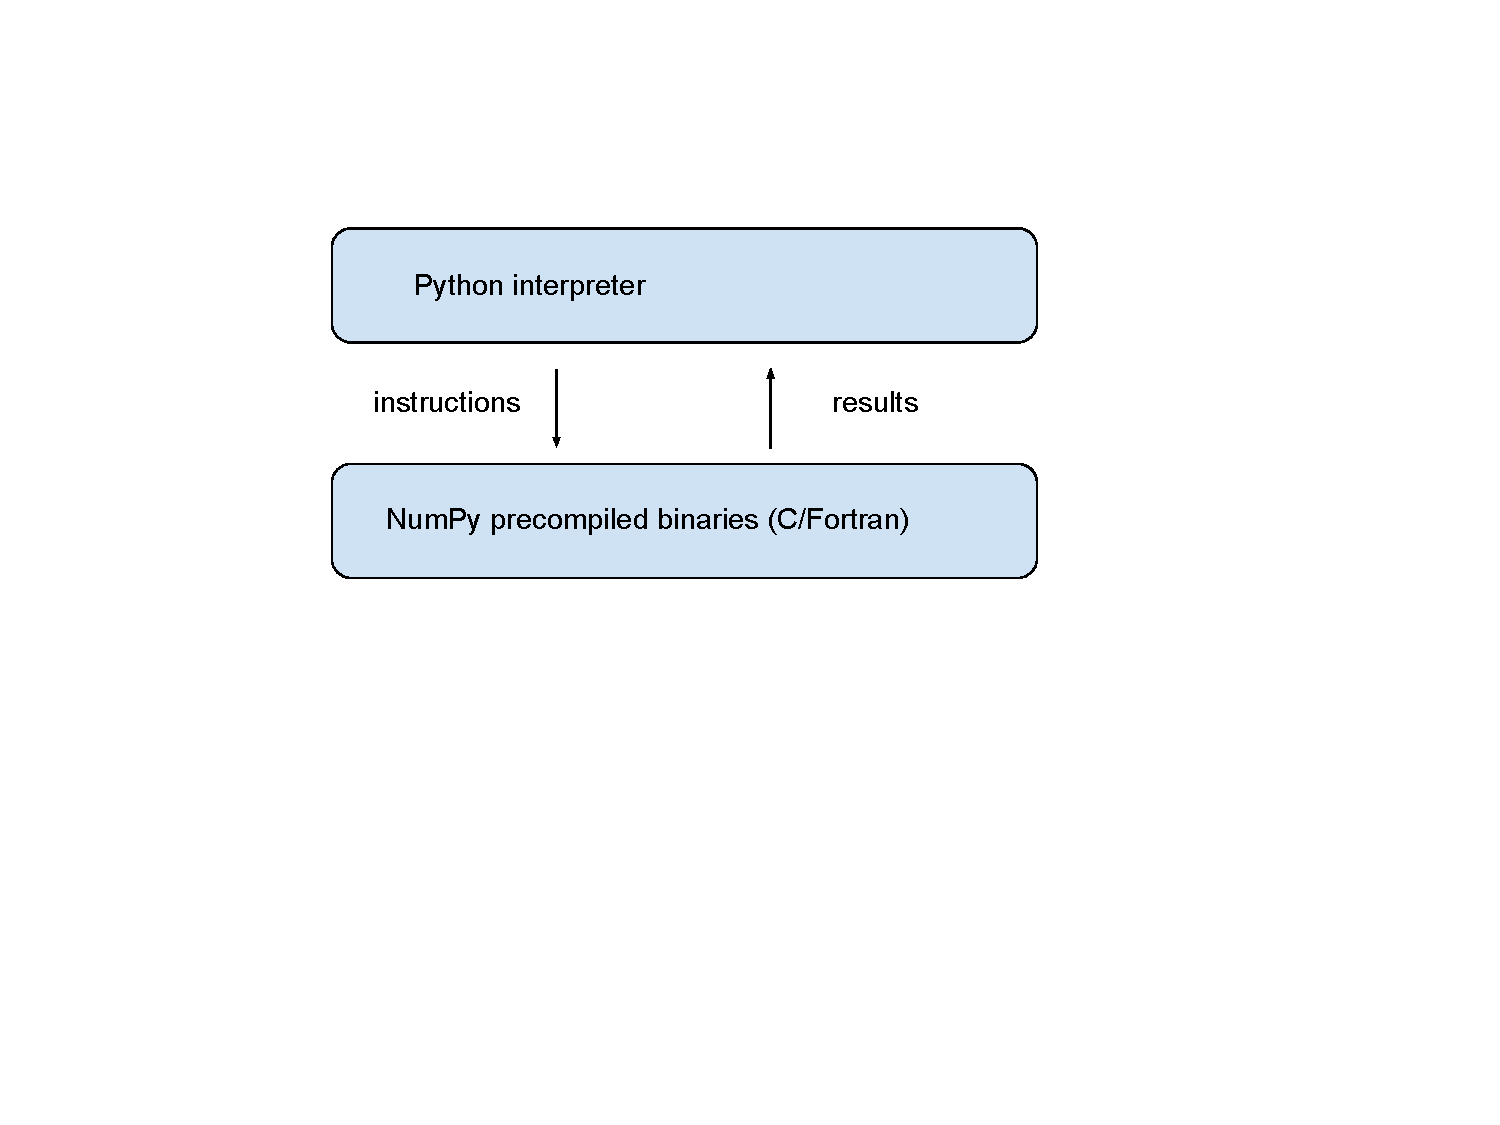
\includegraphics[trim={2cm 8cm 6cm 3cm},clip]{numpy.pdf}}
       \end{center}
    \end{figure}

\end{frame}

\begin{frame}[fragile]

    \begin{minted}{python}
        import numpy 

        A = ((2.0, -1.0),
             (5.0, -0.5))

        b = (0.5, 1.0)

        A, b = np.array(A), np.array(b)

        x = np.inv(A) @ b
    \end{minted}

\end{frame}

\begin{frame}
    
    \begin{enumerate}
        \item Arrays defined with high-level commands 
        \vspace{0.5em}
        %
        \begin{itemize}
            \item (Python / NumPy API)
        \end{itemize}
        %
        \vspace{0.5em}
        \item Execution takes place in an efficient low-level environment
        \vspace{0.5em}
        %
        \begin{itemize}
            \item Efficient machine code (compiled C / Fortran)
        \end{itemize}
        %
        \vspace{0.5em}
        \item Results are returned to the high-level interface
    \end{enumerate}

\end{frame}


\begin{frame}
    \frametitle{MATLAB}

    NumPy is similar to and borrows from the older MATLAB programming
    environment

    \vspace{0.5em}
    \vspace{0.5em}
    \begin{figure}
       \begin{center} % l b r t
        \scalebox{.6}{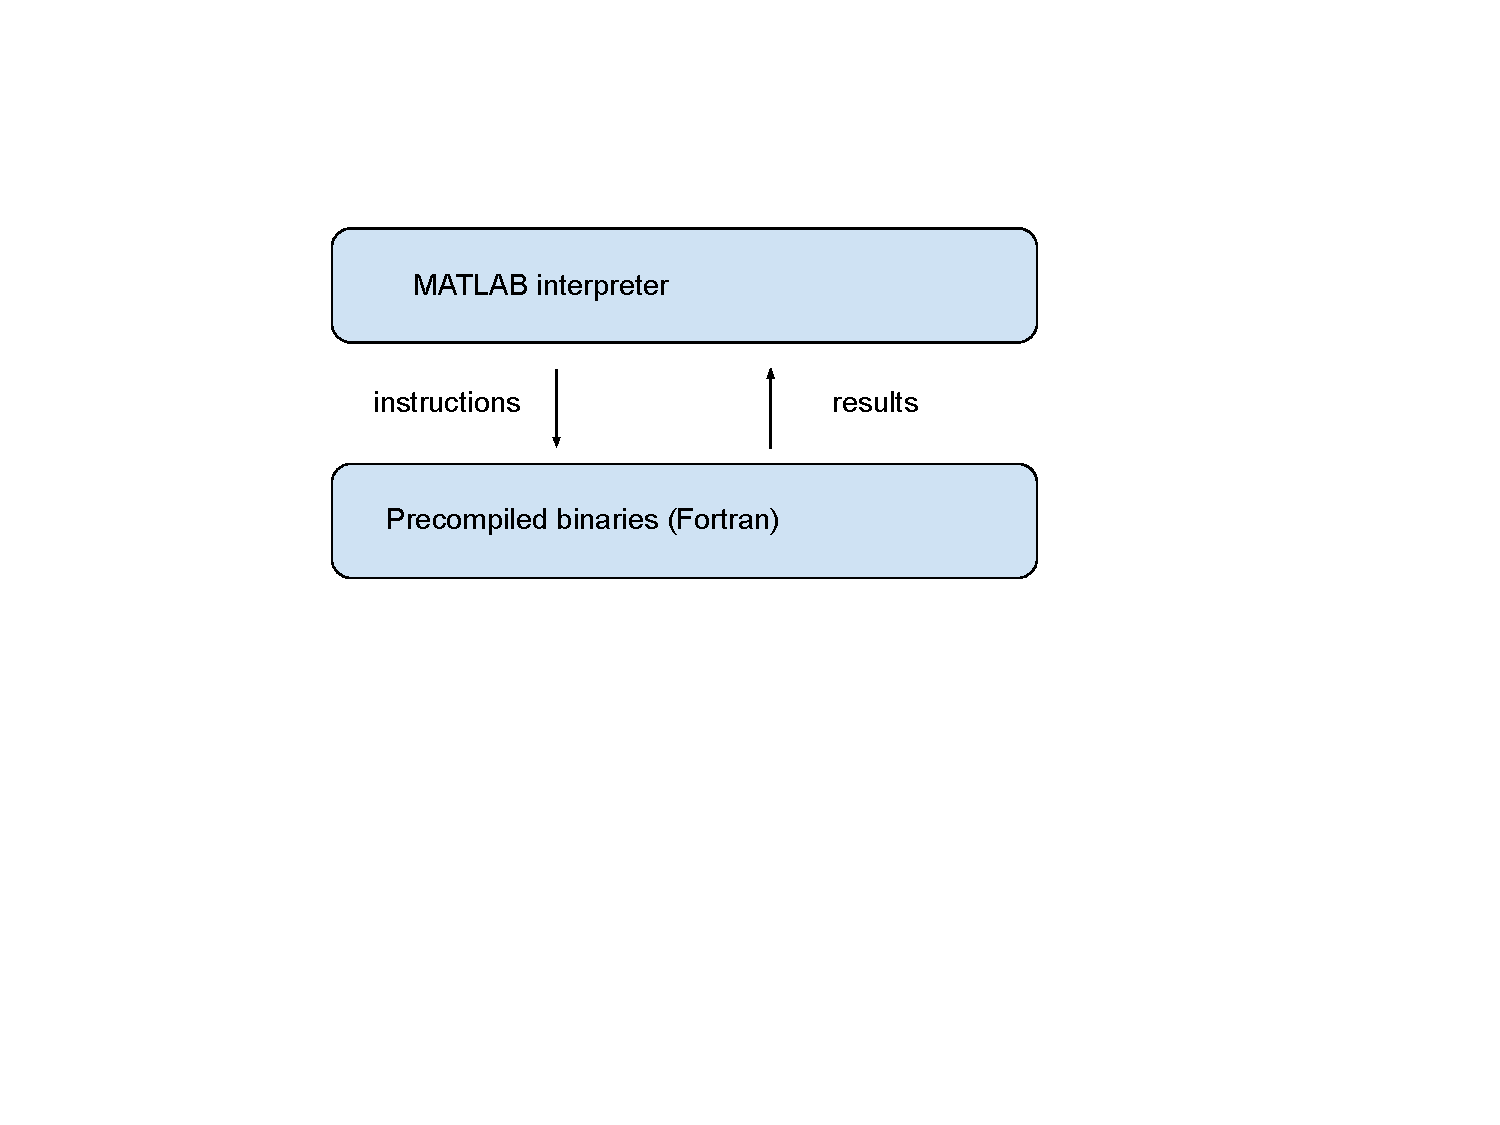
\includegraphics[trim={2cm 8cm 6cm 3cm},clip]{matlab.pdf}}
       \end{center}
    \end{figure}


\end{frame}


\begin{frame}[fragile]
    
    \begin{minted}{matlab}
        A = [2.0, -1.0
             5.0, -0.5];

        b = [0.5, 1.0]';

        x = inv(A) * b
    \end{minted}
    
\end{frame}



    

\begin{frame}
    
    Advantages of NumPy / MATLAB

    \vspace{0.5em}
    \begin{itemize}
        \item Operations are passed to specialized machine code 
        \vspace{0.5em}
        \item Type-checking is paid per array, not per array element
    \end{itemize}

    \vspace{0.5em}
    \vspace{0.5em}
    Disadvantages 

    \begin{itemize}
        \item Can be highly memory intensive (intermediate arrays)
        \vspace{0.5em}
        \item \underline{Fails} to specialize on array \emp{shapes}
        \vspace{0.5em}
        \item Limited --- how would you accelerate the Solow code using NumPy?
    \end{itemize}

\end{frame}







\begin{frame}[fragile]
    \frametitle{Julia --- rise of the JIT compilers}

    Can do MATLAB / NumPy style vectorized operations

    \begin{minted}{julia}
A = [2.0  -1.0
     5.0  -0.5]

b = [0.5  1.0]'

x = inv(A) * b
    \end{minted}
    

    \vspace{0.5em}
    \vspace{0.5em}
    But also has fast loops via an efficient JIT compiler

\end{frame}


\begin{frame}
    
    \Eg Suppose, again, that we want to compute 
    %
    \begin{equation*}
        k_{t+1} = s k_t^\alpha + (1 - \delta) k_t
    \end{equation*}
    %
    from some given $k_0$ 


    \vspace{0.5em}
    \vspace{0.5em}
    \vspace{0.5em}
    \vspace{0.5em}
    \begin{itemize}
        \item Iterative, not easily vectorized
    \end{itemize}

\end{frame}


\begin{frame}[fragile]
    
    \begin{minted}{julia}

function solow(k0, α=0.4, δ=0.1, n=1_000)
    k = k0
    for i in 1:(n-1)
        k = s * k^α + (1 - δ) * k
    end
    return k
end

solow(0.2)  # JIT-compiled at first call
    \end{minted}

    \vspace{0.5em}
    \vspace{0.5em}
    \vspace{0.5em}
    \vspace{0.5em}

    Julia accelerates \texttt{solow} at runtime via a JIT compiler

\end{frame}


\begin{frame}
    
    Pros:

    \begin{itemize}
        \item fast execution --- assuming correct type inference
        \vspace{0.2em}
        \item dynamically typed\ldots (but compiler wants type stability)
        \vspace{0.2em}
        \item close to the maths
    \end{itemize}

        \vspace{0.2em}
        \vspace{0.2em}
        \vspace{0.2em}
        \vspace{0.2em}
        \vspace{0.2em}
        \vspace{0.2em}
    Cons:

    \begin{itemize}
        \item Everything compiled might not be optimal 
        \vspace{0.2em}
        \begin{itemize}
            \item debugging is more challenging
            \vspace{0.2em}
            \item slow first runs
            \vspace{0.2em}
        \end{itemize}
        \item Package instability
        \vspace{0.2em}
        \item Repeated breaking changes
    \end{itemize}

\end{frame}

\begin{frame}[fragile]
    \frametitle{Python + Numba --- same architecture, same speed}
    
    \begin{minted}{python}
from numba import jit

@jit(nopython=True)
def solow(k0, α=0.4, δ=0.1, n=1_000):
    k = k0
    for i in range(n-1):
        k = s * k**α + (1 - δ) * k
    return k

solow(0.2)
    \end{minted}


    Runs at same speed as Julia / C / Fortran

\end{frame}


\begin{frame}
    
    OK, let's talk about the next generation\ldots

\end{frame}


\begin{frame}

    \begin{figure}
       \centering
       \scalebox{0.4}{
\includegraphics{logo.pdf}}
    \end{figure}
    
            \vspace{0.5em}

    \begin{center}
        \url{https://jax.readthedocs.io/en/latest/}
    \end{center}

\end{frame}

\begin{frame}
    
    A high-performance numerical computing library 

            \vspace{0.5em}
            \vspace{0.5em}

    \begin{itemize}
        \item Developed by \href{https://research.google/}{Google Research}
            (prev.\ Google Brain)
            \vspace{0.5em}
        \item NumPy-style API for array operations
            \vspace{0.5em}
        \item GPU/TPU acceleration 
            \vspace{0.5em}
        \item Automatic differentiation
            \vspace{0.5em}
        \item Math-centric library semantics
            \vspace{0.5em}
        \item Rising popularity among ML researchers
    \end{itemize}

            \vspace{0.5em}
            \vspace{0.5em}

    ``The JAX compiler aims to enable researchers to write Python programs\ldots
        that are automatically compiled and scaled to leverage accelerators and
        supercomputers''

\end{frame}

\begin{frame}
    
    \Eg AlphaFold3 is built with Google JAX

        \vspace{0.5em}

    \begin{figure}
       \begin{center} % l b r t
        \scalebox{.24}{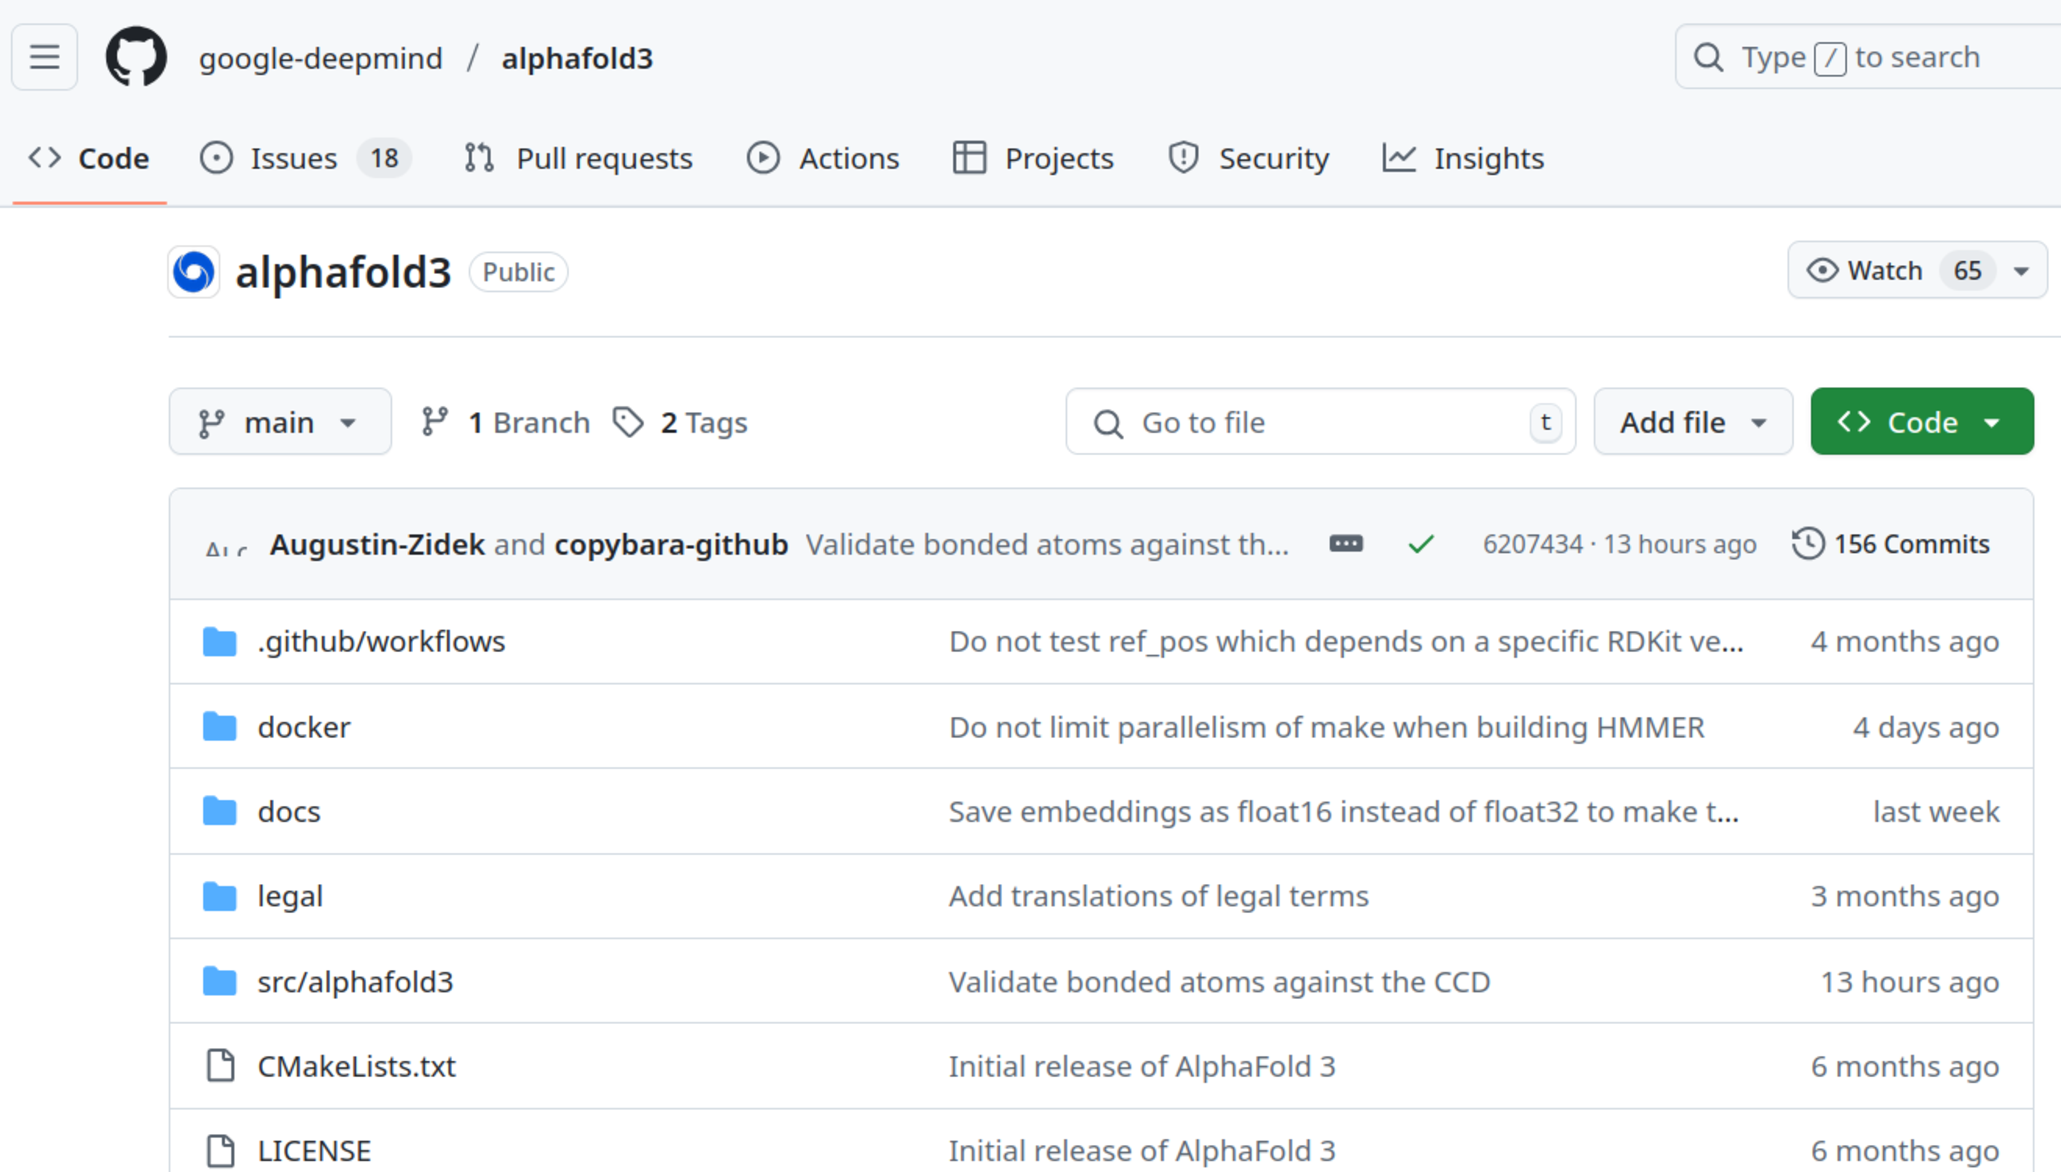
\includegraphics{af.pdf}}
       \end{center}
    \end{figure}


\end{frame}

\begin{frame}
    
    \textbf{Highly accurate protein structure prediction with AlphaFold}

        \vspace{0.5em}
    John Jumper, Richard Evans, Alexander Pritzel, Tim Green, Michael Figurnov,
    Olaf Ronneberger, Kathryn Tunyasuvunakool,\ldots 

        \vspace{0.5em}
    \underline{Nature} Vol.\ 596 (2021)

    \vspace{0.5em}
    \vspace{0.5em}
    \vspace{0.5em}
    \vspace{0.5em}
    \begin{itemize}
        \item Citation count $= ~35$K
        \vspace{0.5em}
        \item Nobel Prize in Chemistry 2024
    \end{itemize}

\end{frame}


\begin{frame}

    ``The acronym JAX stands for \brown{Just After eXecution}''

    \begin{itemize}
        \item monitor function execution once and then compile
    \end{itemize} 

            \vspace{0.5em}
            \vspace{0.5em}
            \vspace{0.5em}

    Another acronym:

    \begin{itemize}
        \item \brown{J}ust-in-time compilation
            \vspace{0.5em}
        \item \brown{A}utomatic differentiation
            \vspace{0.5em}
        \item \brown{X}LA (accelerated linear algebra)
    \end{itemize}



\end{frame}

\begin{frame}[fragile]
    \frametitle{Familiar NumPy-style array API}

    \begin{minted}{python}
        import jax.numpy as jnp

        A = ((2.0, -1.0),
             (5.0, -0.5))

        b = (0.5, 1.0)

        A, b = jnp.array(A), jnp.array(b)

        x = jnp.inv(A) @ b
    \end{minted}

\end{frame}


\begin{frame}[fragile]
    \frametitle{Accelerated linear algebra (XLA)}

    Array operations are
    %
    \begin{itemize}
        \item sent to precompiled XLA device code that takes array shapes as a
            parameter
        \vspace{0.5em}
        \item automatically parallelized 
        \vspace{0.5em}
        \item automatically optimized for and deployed to available hardware
    \end{itemize}

\end{frame}


\begin{frame}[fragile]
    \frametitle{Explicit just-in-time compilation}
    
    \begin{minted}{python}
@jax.jit
def f(x):
    term1 = 2 * jnp.sin(3 * x) * jnp.cos(x/2)
    term2 = 0.5 * x**2 * jnp.cos(5*x) / (1 + 0.1 * x**2)
    term3 = 3 * jnp.exp(-0.2 * (x - 4)**2) * jnp.sin(10*x)
    return term1 + term2 + term3 
    \end{minted}

    \vspace{0.5em}
    \vspace{0.5em}

    \begin{itemize}
        \item Compiles at first call (e.g., \texttt{result = f(x)})
        \item Compiler specializes on \brown{both} shape and data type
    \end{itemize}

\end{frame}


\begin{frame}

    Precompiled vs compiled in JAX:

    \begin{figure}[h!]
        \centering
        \scalebox{0.45}{\begin{tikzpicture}[
    scale=0.2,
    node distance=1.5cm,
    block/.style={rectangle, draw, fill=white, text width=3.5cm, align=center, rounded corners, minimum height=1cm, font=\sffamily},
    process/.style={rectangle, draw, fill=white, text width=3.5cm, align=center, rounded corners, minimum height=1cm, font=\sffamily},
    compiler/.style={rectangle, draw, fill=compilerpurple!20, text width=4cm, align=center, rounded corners, minimum height=1.5cm, font=\sffamily},
    kernel/.style={ellipse, draw, fill=xlagreen!20, text width=3cm, align=center, minimum height=1cm, font=\sffamily},
    device/.style={rectangle, draw, fill=devicegray!20, text width=6cm, align=center, minimum height=1.5cm, font=\sffamily\bfseries, rounded corners},
    arrow/.style={-Latex, thick, jaxblue},
    label_text/.style={font=\sffamily\small, text=black},
    title_box/.style={rectangle, fill=jaxblue!10, rounded corners, inner sep=5pt, font=\sffamily\bfseries, align=center}
]

    % Left Path: Simple Operations
    \node (python_simple) [block, fill=pythonorange!20] {Python Code: \\ `x + y`};
    \node (jax_dispatch_simple) [process, below=of python_simple] {JAX Dispatch \\ (for each op)};
    \node (xla_kernel_add) [kernel, below=of jax_dispatch_simple] {Precompiled XLA kernel (Add)};
    % Removed xla_kernel_mul and xla_kernel_sub nodes

    % Right Path: JIT-Compiled Operations
    \node (python_jit) [block, fill=pythonorange!20, right=4cm of python_simple] {Python Function: \\ `@jax.jit \\ def func(x, y): \\ \quad return x + y * 2`};
    \node (jax_tracing) [process, fill=tracingyellow!20, below=of python_jit] {JAX Tracing \\ (to Jaxpr IR)};
    \node (xla_compiler) [compiler, below=of jax_tracing] {XLA JIT Compiler \\ (Master Builder)};
    \node (fused_kernel) [kernel, fill=xlagreen!40, below=of xla_compiler] {Fused XLA kernel \\ (optimized for `func`)};

    % Device Execution (Common End Point)
    % Adjusted positioning for device node due to removed kernels
    \node (device) [device, below=3cm of $(xla_kernel_add.south)!0.2!(fused_kernel.south)$] {Device Execution \\ (CPU / GPU / TPU)};

    % Arrows for Simple Operations
    \draw [arrow] (python_simple) -- (jax_dispatch_simple);
    \draw [arrow] (jax_dispatch_simple) -- (xla_kernel_add);
    \draw [arrow] (xla_kernel_add) -- (device);
    % Removed dashed arrows to xla_kernel_mul and xla_kernel_sub

    % Arrows for JIT-Compiled Operations
    \draw [arrow] (python_jit) -- (jax_tracing);
    \draw [arrow] (jax_tracing) -- (xla_compiler);
    \draw [arrow] (xla_compiler) -- (fused_kernel);
    \draw [arrow] (fused_kernel) -- (device);

    \node [label_text, right=0.6cm of xla_compiler.north east, anchor=south
    west, text width=5cm] {Builds a custom, optimized kernel using existing, generic kernels};

    % Fit boxes for visual grouping
    % Adjusted fit box for simple path
    \node[fit=(python_simple)(xla_kernel_add)(jax_dispatch_simple), draw, dashed, inner sep=10pt, label_text, label={[label_text]above:individual dispatch}] (simple_path_box) {};
    \node[fit=(python_jit)(fused_kernel)(jax_tracing), draw, dashed, inner sep=10pt, label_text, label={[label_text]above:function compilation}] (jit_path_box) {};
\end{tikzpicture}

}
    \end{figure}
    
\end{frame}



\begin{frame}
    
    JIT compiler tools for optimization

    \begin{itemize}
        \item Operations combined into fused kernels for GPU/TPU
        \vspace{0.5em}
        \item Eliminate intermediate buffers / memory writes and reads
        \vspace{0.5em}
        \item Loop unrolling
        \vspace{0.5em}
        \item Specialized algorithms
        \vspace{0.5em}
        \item Memory layout optimization for multi-dimensional arrays
    \end{itemize}

        \vspace{0.5em}
        \vspace{0.5em}
    ``JAX's JIT compiler acts like a master engineer''

\end{frame}



\begin{frame}[fragile]
    \frametitle{Automatic differentiation}
    
    \vspace{-1em}
    \begin{minted}{python}
import jax.numpy as jnp
from jax import grad, jit

def f(θ, x):
  for W, b in θ:
    w = x @ W + b
    x = jnp.tanh(w)  
  return x

def loss(θ, x, y):
  return jnp.sum((y - f(θ, x))**2)

grad_loss = jit(grad(loss))  # Now use gradient descent 
    \end{minted}

\end{frame}



\begin{frame}{Features of JAX}

    Let's review some other features

        \vspace{0.5em}

    \begin{itemize}
        \item Functional programming
        \vspace{0.5em}
        \item PyTrees
    \end{itemize}
    
\end{frame}

\begin{frame}
    \frametitle{Functional Programming}
    
    JAX adopts a \underline{functional programming style}

    \vspace{0.5em}
    \vspace{0.5em}
    \vspace{0.5em}
    \vspace{0.5em}
    Key feature: \emp{functions are pure!}

    \begin{itemize}
        \item Deterministic: same input $\implies$ same output 
        \vspace{0.5em}
        \item Have no side effects (don't modify state outside their scope)
    \end{itemize}


        \vspace{0.5em}
        \vspace{0.5em}
        \vspace{0.5em}
    Functional programming usually adopts immutable data

\end{frame}


\begin{frame}[fragile]

    A \brown{non-pure} function
    \vspace{0.5em}
    \vspace{0.5em}

    \begin{minted}{python}
tax_rate = 0.1 
prices = [10.0, 20.0] 

def add_tax(prices):
    for i, price in enumerate(prices):
        prices[i] = price * (1 + tax_rate)    
    print('Modified prices: ', prices)
    \end{minted}

    \vspace{0.5em}
    \vspace{0.5em}
    \vspace{0.5em}
    Why is this not pure?
    
\end{frame}



\begin{frame}[fragile]

    A \brown{pure} function
    \vspace{0.5em}
    \vspace{0.5em}

    \begin{minted}{python}
tax_rate = 0.1 
prices = [10.0, 20.0] 

def add_tax_pure(prices, tax_rate):
    return [price * (1 + tax_rate) for price in prices]
    \end{minted}
    
\end{frame}


\begin{frame}

    General advantages:

    \begin{itemize}
        \item Helps testing: each function can operate in isolation
    \vspace{0.5em}
        \item Data dependencies are explicit, which helps with understanding and optimizing complex computations 
    \vspace{0.5em}
        \item Promotes deterministic behavior and hence reproducibility
    \vspace{0.5em}
        \item Prevents bugs that arise from mutating shared state
    \end{itemize}

\end{frame}



\begin{frame}
    
    Advantages for JAX:

     \begin{itemize}
         \item Pure functions are easier to differentiate 
        \vspace{0.5em}
         \item Pure functions are easier to parallelize and optimize (don't
             depend on shared mutable state)
        \vspace{0.5em}
         \item Transformations can be composed cleanly (predictable results)
     \end{itemize}


\end{frame}

\begin{frame}
    \frametitle{JAX PyTrees}

    A tree-like data structure built from Python containers

    \vspace{0.5em}
    A concept, not a data type

    \vspace{0.5em}
    \vspace{0.5em}
    \vspace{0.5em}
    \Egs

    \begin{itemize}
        \item A list of dictionaries, each dictionary contains parameters
        \item A dictionary of lists 
        \item A dictionary of lists of dictionaries
        \item etc.
    \end{itemize}

\end{frame}


\begin{frame}
    
    
    \resizebox{0.9\textwidth}{!}{
        % JAX PyTree TikZ Diagram with Pygments Syntax Highlighting
% To use this in your LaTeX document:
% 1. Ensure you have the required packages in your preamble: tikz, minted, varwidth
% 2. Load TikZ libraries: shapes, arrows, positioning, fit, backgrounds, calc
% 3. Define the colors and minted settings in your preamble
% 4. Place this code inside a figure environment

% Required packages for your preamble:
% \usepackage{tikz}
% \usepackage{minted}
% \usepackage{varwidth}
% \usetikzlibrary{shapes,arrows,positioning,fit,backgrounds,calc}

% Color definitions for your preamble:
% \definecolor{containerblue}{RGB}{66, 133, 244}
% \definecolor{leafgreen}{RGB}{52, 168, 83}
% \definecolor{textgray}{RGB}{51, 51, 51}
% \definecolor{backgroundgray}{RGB}{248, 249, 250}
% \definecolor{codebg}{RGB}{241, 241, 241}

% Minted settings for your preamble:
% \setminted[python]{
%   fontsize=\small,
%   baselinestretch=1.2,
%   bgcolor=codebg,
%   linenos=false,
%   breaklines=true,
%   frame=none
% }

% Place the following code in your document inside a figure environment:
% \begin{figure}
%   \centering
%   ... code below ...
%   \caption{JAX PyTree Structure Visualization}
%   \label{fig:jax-pytree}
% \end{figure}

\begin{tikzpicture}[
    % Node styles
    container/.style={draw=containerblue!70!black, fill=containerblue, rounded corners=3pt, minimum width=3cm, minimum height=1cm, text=white, font=\sffamily\bfseries},
    leaf/.style={draw=leafgreen!70!black, fill=leafgreen, rounded corners=3pt, minimum width=2cm, minimum height=1cm, text=white, font=\sffamily\bfseries},
    label/.style={font=\sffamily\small, text=textgray},
    level distance=2cm,
    sibling distance=3cm
]

% Background
\node[rectangle, fill=backgroundgray, minimum width=20cm, minimum height=15cm] (background) at (0,0) {};

% Title
\node[font=\sffamily\bfseries\Large, text=textgray] at (0,6.5) {JAX PyTree Structure};

% Sample code with syntax highlighting
\node[anchor=north] (code) at (0,5.5) {
  \begin{varwidth}{14cm}
    \begin{minted}{python}
pytree = {
    "a": [1, 2, 3],
    "b": {"c": jnp.array([4, 5]), "d": jnp.array([[6, 7], [8, 9]])}
}
    \end{minted}
  \end{varwidth}
};

% Add a border around the code
\begin{scope}[on background layer]
\draw[rounded corners=3pt, draw=black!20] 
  ([shift={(-0.5em,-0.5em)}]code.south west) rectangle 
  ([shift={(0.5em,0.5em)}]code.north east);
\end{scope}

\path (code.south) -- ++(0,-1.5) coordinate (after_code);

\node[container] (root) at (0,2) {dict};

% First level children
\node[container] (list) at (-4,1) {list};
\node[label] at (-4,1.8) {"a"};
\node[container] (dict) at (4,1) {dict};
\node[label] at (4,1.8) {"b"};

% Second level - list elements
\node[leaf] (n1) at (-6,-1) {1};
\node[leaf] (n2) at (-4,-1) {2};
\node[leaf] (n3) at (-2,-1) {3};

% Second level - dict elements
\node[container] (array1) at (2,-1) {array};
\node[label] at (2,-0.2) {"c"};
\node[container] (array2) at (6,-1) {array};
\node[label] at (6,-0.2) {"d"};

% Array values (leaf nodes)
\node[leaf, text width=2.5cm, align=center] (val1) at (2,-3) {[4, 5]};
\node[leaf, text width=3cm, align=center] (val2) at (6,-3) {[[6, 7], [8, 9]]};

% Edges connecting nodes
\draw[->, >=stealth, thick, textgray] (root) -- (list);
\draw[->, >=stealth, thick, textgray] (root) -- (dict);
\draw[->, >=stealth, thick, textgray] (list) -- (n1);
\draw[->, >=stealth, thick, textgray] (list) -- (n2);
\draw[->, >=stealth, thick, textgray] (list) -- (n3);
\draw[->, >=stealth, thick, textgray] (dict) -- (array1);
\draw[->, >=stealth, thick, textgray] (dict) -- (array2);
\draw[->, >=stealth, thick, textgray] (array1) -- (val1);
\draw[->, >=stealth, thick, textgray] (array2) -- (val2);

% Legend
\node[container, minimum width=1cm, minimum height=0.6cm] (legend1) at (-7,-5) {};
\node[text=textgray, font=\sffamily, anchor=west] at (-6.5,-5) {Container nodes (dict, list, tuple)};

\node[leaf, minimum width=1cm, minimum height=0.6cm] (legend2) at (-7,-6) {};
\node[text=textgray, font=\sffamily, anchor=west] at (-6.5,-6) {Leaf nodes (arrays, scalars)};

% Additional explanation
\node[text=textgray, font=\sffamily\bfseries, align=center] at (0,-4.5) {JAX PyTrees: Nested containers with leaves as arrays or scalars};

\end{tikzpicture}

    }

\end{frame}


\begin{frame}
    
    JAX can

    \begin{itemize}
        \item apply functions to all leaves in a PyTree structure
        \vspace{0.5em}
        \item differentiate functions with respect to the leaves of PyTrees
        \vspace{0.5em}
        \item etc.
    \end{itemize}


\end{frame}

\begin{frame}
    

\begin{figure}
\centering
\begin{tikzpicture}[
  scale=0.5, transform shape, % Scale down the entire figure
  level distance=1.5cm,
  level 1/.style={sibling distance=2.5cm},
  level 2/.style={sibling distance=2cm},
  every node/.style={draw, rounded corners, fill=white, drop shadow, align=center, font=\sffamily},
  edge from parent/.style={thick, draw, -{Stealth[length=6pt]}},
  pytree/.style={draw, rounded corners, fill=blue!10, minimum width=1.8cm, minimum height=0.9cm},
  pytree2/.style={draw, rounded corners, fill=green!10, minimum width=1.8cm, minimum height=0.9cm},
  result/.style={draw, rounded corners, fill=purple!10, minimum width=1.8cm, minimum height=0.9cm},
  operation/.style={draw, circle, fill=red!20, inner sep=2pt}
]

% First pytree - unchanged
\node[pytree] (root1) at (-5,0) {pytree1};
\node[pytree, below left=1.5cm and 1.2cm of root1] (a1) {\texttt{'a'}: [1, 2, 3]};
\node[pytree, below right=1.5cm and 1.2cm of root1] (b1) {\texttt{'b'}: dict};
\node[pytree, below left=1.5cm and 0.4cm of b1] (c1) {\texttt{'c'}: [4, 5, 6]};
\node[pytree, below right=1.5cm and 0.4cm of b1] (d1) {\texttt{'d'}: 7};

\draw[edge from parent] (root1) -- (a1);
\draw[edge from parent] (root1) -- (b1);
\draw[edge from parent] (b1) -- (c1);
\draw[edge from parent] (b1) -- (d1);

% Second pytree - unchanged
\node[pytree2] (root2) at (5,0) {pytree2};
\node[pytree2, below left=1.5cm and 1.2cm of root2] (a2) {\texttt{'a'}: [10, 20, 30]};
\node[pytree2, below right=1.5cm and 1.2cm of root2] (b2) {\texttt{'b'}: dict};
\node[pytree2, below left=1.5cm and 0.4cm of b2] (c2) {\texttt{'c'}: [40, 50, 60]};
\node[pytree2, below right=1.5cm and 0.4cm of b2] (d2) {\texttt{'d'}: 70};

\draw[edge from parent] (root2) -- (a2);
\draw[edge from parent] (root2) -- (b2);
\draw[edge from parent] (b2) -- (c2);
\draw[edge from parent] (b2) -- (d2);


% Result pytree - shifted down from -6 to -7.5
\node[result] (rootR) at (0,-7.5) {result};
\node[result, below left=1.5cm and 1.2cm of rootR] (aR) {\texttt{'a'}: [11, 22, 33]};
\node[result, below right=1.5cm and 1.2cm of rootR] (bR) {\texttt{'b'}: dict};
\node[result, below left=1.5cm and 0.4cm of bR] (cR) {\texttt{'c'}: [44, 55, 66]};
\node[result, below right=1.5cm and 0.4cm of bR] (dR) {\texttt{'d'}: 77};

\draw[edge from parent] (rootR) -- (aR);
\draw[edge from parent] (rootR) -- (bR);
\draw[edge from parent] (bR) -- (cR);
\draw[edge from parent] (bR) -- (dR);

% Arrows from input pytrees to result - adjusted for new result position
%\draw[-{Stealth[length=6pt]}, thick, dashed, red] (root1) to[out=-30, in=150] (rootR);
%\draw[-{Stealth[length=6pt]}, thick, dashed, red] (root2) to[out=-150, in=30] (rootR);


\end{tikzpicture}
\caption{\texttt{jax.tree.map(lambda x, y: x + y, pytree1, pytree2)}}
\end{figure}

\end{frame}


\begin{frame}[fragile]
    
    \begin{minted}{python}
# Apply gradient updates to all parameters
def sgd_update(params, grads, learning_rate):
    return jax.tree.map(
        lambda p, g: p - learning_rate * g, 
        params, 
        grads
    )

# Calculate gradients (PyTree with same structure as params)
grads = jax.grad(loss_fn)(params, inputs, targets)

# Update all parameters at once
updated_params = sgd_update(params, grads, 0.01)    
    \end{minted}

\end{frame}


\begin{frame}{Summary}
    
    Advantages over NumPy / MATLAB

    \vspace{0.5em}
    \begin{itemize}
        \item Can specialize machine code to data types \textbf{and} shapes!
        \vspace{0.5em}
        \vspace{0.5em}
        \item Automatically matches tasks with accelerators
        \vspace{0.5em}
        \vspace{0.5em}
        \item Same code, multiple backends (CPUs, GPUs, TPUs)
        \vspace{0.5em}
        \vspace{0.5em}
        \item Can fuse array operations for speed and memory efficiency
        \vspace{0.5em}
        \vspace{0.5em}
        \item Integrated efficient autodiff
    \end{itemize}

\end{frame}

\begin{frame}

    Advantages of JAX (vs PyTorch / Tensorflow / etc.) for economists:
    %
    \begin{itemize}
        \item elegant functional programming style -- close to maths
            \vspace{0.5em}
        \item elegant autodiff tools
            \vspace{0.5em}
        \item array operations follow standard NumPy API
    \end{itemize}

            \vspace{0.5em}
            \vspace{0.5em}

    Exposes low level functions / fewer off-the-shelf solutions

\end{frame}


\end{document}
